\documentclass[10pt]{article}

\usepackage[margin=1in]{geometry}
\usepackage{textcomp}
\usepackage{parskip}
\usepackage{amsmath}
\usepackage[backend=biber, style=alphabetic, sorting=ynt]{biblatex}
\usepackage{graphicx}
\graphicspath{{./images/}}
\usepackage{wrapfig}

\addbibresource{paper.bib}

\begin{document}

\section{Introduction}

\subsection{Objective}

In experiments for dark matter detection, one of the most important and challenging hurdles to overcome is that of background radiation. Unwanted particles from a variety of sources can produce event signatures that appear very similar to those of dark matter candidates. In the PICO-60 bubble chamber experiment for detection of weakly interacting massive particles (WIMPs), these came in the form of neutrons (from unknown sources) and alpha particles (from decay of radon and associated daughter isotopes).

To resolve this, physicists must determine a discriminator function that can, based on some sensory data, separate dark matter candidates from background radiation. Two general problems stand in the way:

\begin{enumerate}
    \item A detailed simulation of the physical environment is often used to produce an accurate discriminator. This takes a long time even for a team of experienced physicists, and will have to be updated whenever the physical variables of the experimental apparatus change.
    \item The primary intention of many dark matter experiments, which is to reduce background radiation to the lowest level possible, means that there will be a very small number of background events detected. This places a severe limit on the amount of data that is available to optimize such a discriminator.
    \item Furthermore, what little data is available to optimize a discriminator very often contains impurities, because whatever background radiation is present during WIMP detection runs is also present during calibration runs. These are difficult to separate without already having access to a functional discriminator, creating a ``chicken or the egg'' problem (from which the most common way to escape is to create a time- and labor-intensive simulation).
    \item When a discriminator is optimized on the impure training data available, for which ground truths are defined based on the calibration run of origin, it is really being optimized to discriminate between calibration runs, rather than between classes of particles. Without careful consideration, these two goals may not match up. For instance, a discriminator can undesirably fit on noise that varies between calibration runs.
\end{enumerate}

The objective of this study is to solve all 3 of these problems using machine learning. This is done using semi-supervised algorithms that simultaneously learn an effective discriminator and improves the purity of their own training data sets.

\subsection{Hyperparameter Optimization}

Learning algorithms in this study are optimized using grid searches, in which many different combinations of hyperparameters are tested. The computational work required for a grid search increases exponentially with the number of hyperparameters $n$ and the number of options per hyperparameter $m$; to be exact, its complexity is $O(m^{n})$. Thus, it is important to minimize the number of hyperparameters that are optimized at once.

Since the semi-supervised learning algorithms used incorporate  neural network models, optimization is a much simpler task if the network's hyperparameters are already optimized. Thus, the optimization task is split into two distinct phases:

\begin{enumerate}
    \item Optimize the hyperparameters of a neural network on validation accuracy, to accurately reproduce the imperfect ground truths it is trained on. While this does not produce an optimal discriminator, it does reveal architectures that are capable, in essence, of learning to accomplish the discrimination task.
    \item Using neural network hyperparameters that were determined to be effective, optimize the hyperparameters of the semi-supervised learning algorithm to reproduce Acoustic Parameter as closely as possible. Since Acoustic Parameter is not used to optimize the neural network directly at any point, models that excel at this task demonstrate an ability to learn the desired discriminator while ignoring the impurities in the training set.
\end{enumerate}

\subsection{Existing Work}

During PICO-60 analysis, a function known as Acoustic Parameter was derived from simulations. It discriminates between alpha particles and nuclear recoils based on audio data (specifically the banded Fourier transform $\beta_{8}$, which is detailed in section \textbf{2.1.2}).

WIMP candidates in the cross-section and mass ranges that the PICO-60 detector is sensitive to are predicted to produce nuclear recoils with the same properties as those created by neutrons. The key difference is that neutrons frequently (but not always) scatter and produce multiple bubbles, where the extremely small predicted cross sections of WIMP candidates mean that they should almost invariably create just one bubble. This means single-bubble neutron events can be used to optimize a discriminator to detect WIMP events.

There was no explicit alpha particle calibration data collected as part of the PICO-60 experiment. However, the previous analysis revealed that there were no WIMP candidates detected. Also, based on the known ratio of multiple- to single-bubble neutron events, it is unlikely that there is more than 1 single-bubble neutron event throughout the background runs. This means they can be used as a high-purity alpha calibration set.

While these two known event sets were only used for minor calibrations of Acoustic Parameter, there is no reason they cannot be used to optimize a machine learning discriminator from scratch.

\section{Data Formats}

Discriminators can use a variety of different data formats to make predictions. These are collected from the two essential sensors present in the PICO-60 apparatus: piezoelectric microphones (piezos) and cameras.

\subsection{Piezo-Derived}

\subsubsection{Raw Waveform}

The lowest-level data derived from the piezos is the raw waveform $\omega$. $\omega$ consists of a series of samples collected every 400,000\textsuperscript{th} of a second. They are each represented as a 16-bit integer. Only the section of the audio between sample 90,000 (inclusive) and sample 190,000 (exclusive) was used during most experiments, because before this there is background noise, and afterwards there is a clipped signal produced by hydraulics repressurizing the vessel. (These sections contain no information and can be undesirably fit on by neural networks.)

\subsubsection{Fourier Transform}

The raw waveform $\omega$ is converted into the frequency domain by means of a 1-dimensional Discrete Fourier Transform for real input. Since DFTs produce sequences of complex numbers, the magnitude of each element is computed. The full-resolution Fourier transform $\beta _{50,000}$ consists of a sequence of complex numbers, half the length of the raw waveform $\omega$.

Beyond this, arbitrary-resolution banded Fourier transforms $\beta _{N<50,001}$ can be computed by integrating the resonant energy over all frequencies within each of a set of bands. They can be thought of as a method of signal downscaling, compressing the signal into a smaller number of data points. Particular band resolutions used include $\beta _{8}$ (which is the input to Acoustic Parameter and initial neural network experiments), $\beta _{5}$, $\beta _{10}$, $\beta _{20}$, and $\beta _{40}$.

\begin{figure}[h]
    \centering
    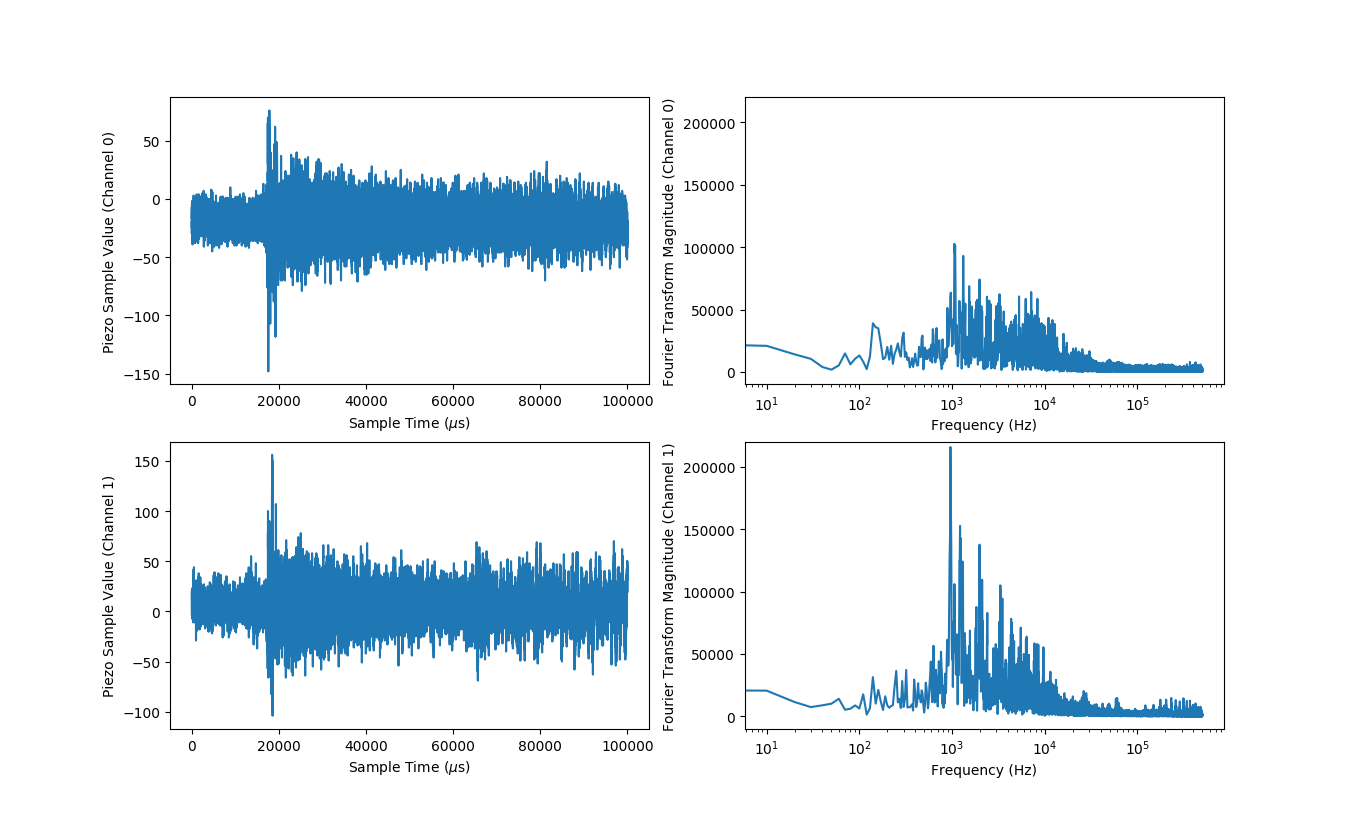
\includegraphics[width=\textwidth]{audio}
    \caption{\label{} An example of the cropped audio waveform $\omega$ and full resolution Fourier transform $\beta_{50,001}$.}
\end{figure}

\subsection{Camera-Derived}

\subsubsection{Image Window Sequence}

For each event that is captured, the 4 cameras within the PICO-60 apparatus each capture a sequence of 71 images before and after formation of a bubble is detected. These raw images contain a large amount of extraneous information; they encompass the entire vessel. To reduce the input information, the image window sequence $\iota$ includes 50\texttimes50 cropped windows around the position of the bubble. The 71 frames, many of which contain either no bubble or a bubble in later stages of formation, are reduced to 10 immediately around the formation of the bubble. $\iota$ includes 5 frames from before the recording trigger, because the bubble does not cause a trigger until it is already at a significant size.

\begin{figure}[h]
    \centering
    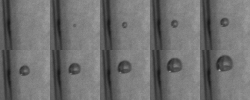
\includegraphics[width=0.7\textwidth]{image_grid}
    \caption{\label{} An example of the image sequence $\iota$.}
\end{figure}

\subsubsection{3D Position}

The 3-dimensional position $\chi$ of the bubble within the vessel is calculated using triangulation, based on the known positions and angles of the cameras and the position of the bubble within the field of view of each camera. This is used in the banded frequency position correction function $PosCor(\beta _{8}, \chi)$, which corrects $\beta _{8}$ for variations in amplitude which depend on the position of the bubble.

\section{Data Cuts}

Techniques in this study are trained and validated on a number of different data sets. The selection of these sets focused on the fundamental trade-off between quality and quantity of data; by setting a higher standard for the validity of training data, one has less data to train on.

The initial data set $D$ to which these cuts are applied consists of all events recorded during PICO-60 run 2.

\subsection{Basic Quality Cut}

A certain number of cuts are necessarily applied to all data to ensure meaningful results. Otherwise, significant overfitting on biases in the data is likely. This basic quality cut $QualCut(D)$ consists of the following restrictions:

\begin{itemize}
    \item The run was not collected during engineering or testing ($\texttt{run\_type}\neq99$)
    \item Recording was triggered by the camera ($\texttt{trigger\_main}=0$)
    \item Acoustic Parameter is not erroneously large and negative ($log_{10}(\texttt{acoustic\_bubnum})>-100$)
    \item Recorded more than 25 seconds after reaching target pressure ($\texttt{te}>25$)
    \item The bubble position $\chi$ was successfully calculated ($[\chi_{X}, \chi_{Y}, \chi_{Z}]\neq[-100, -100, -100]$)
\end{itemize}

\subsection{Bubble Multiplicity Cut}

PICO-60 events which include multiple bubbles are \textit{always} neutron events; alpha particles and WIMP candidates never scatter. Thus, no discriminator is required to handle these events, so they are removed. The bubble multiplicity cut $MultiCut(D)$ consists of the following restrictions:

\begin{itemize}
    \item Either 0 or 1 bubbles are detected based on images from the camera ($\texttt{nbub}<2$)
    \item The number of bubbles approximated using the pressure transducer is close to 1 ($0.7<\texttt{dytranCZ}<1.3$)
\end{itemize}

\subsection{Wall Cut}

Events that occur near the walls of the vessel have acoustic properties which are notably different from events nearer the center of the vessel. It can be desirable for a discriminator to handle these events correctly; however, Acoustic Parameter does not, and neither does the neural network used in the previous PICO-60 paper. Thus, removing wall events allowed for a more meaningful direct comparison between a new neural network and existing techniques.

The complete wall cut $WallCut(D)$ is a composition of the fiducial cut $FidWallCut(D)$ (which makes use of the 3D position $\chi$), the pressure cut $PresWallCut(D)$ (which uses data from the pressure transducer), and the acoustic cut $AcWallCut(D)$ (which uses the banded Fourier transform $\beta _{8}$).

\subsubsection{Fiducial Cut}

The fiducial cut $FidWallCut(D)$ defines an spatial area along the walls of the vessel within which no events are accepted. It makes use of the bubble position $\chi$, the distance from the bubble to the center of the vessel $R$, and the distance from the bubble to the nearest wall, which is defined as $min(\texttt{Dwall}, \texttt{Dwall\_horiz})$. It is defined as follows:

\begin{itemize}
    \item $Z \leq 523$
    \item Any of the following 4 restrictions are true:
    \begin{itemize}
        \item $(min(\texttt{Dwall}, \texttt{Dwall\_horiz}) > 6) \land (0 < \chi_{Z} \leq 400)$
        \item $(min(\texttt{Dwall}, \texttt{Dwall\_horiz}) > 6) \land (\chi_{Z} \leq 0) \land (R \leq 100)$
        \item $(min(\texttt{Dwall}, \texttt{Dwall\_horiz}) > 13) \land (\chi_{Z} \leq 0) \land (R > 100)$
        \item $(min(\texttt{Dwall}, \texttt{Dwall\_horiz}) > 13) \land (\chi_{Z} > 400)$
    \end{itemize}
\end{itemize}

\subsubsection{Pressure Cut}

The pressure cut $PresWallCut(D)$ restricts the pressure detected by the pressure transducer, without any position corrections, to be close to 1 ($0.7<\texttt{dytranC}<1.3$). In combination with the acoustic cut $AcWallCut(D)$, this acts as a backup to the fiducial cut.

\subsubsection{Acoustic Cut}

The acoustic cut $AcWallCut(D)$ is defined using the banded Fourier transform $\beta_{8}$ as follows:

$45 < mean(\beta_{8}[(0, 2), (0, 1)]) < 300$

This takes advantage of differences in the frequency distribution (specifically the first and second frequency bands of the first and third piezos) of wall events and non-wall events.

\begin{figure}[h!]
    \centering
    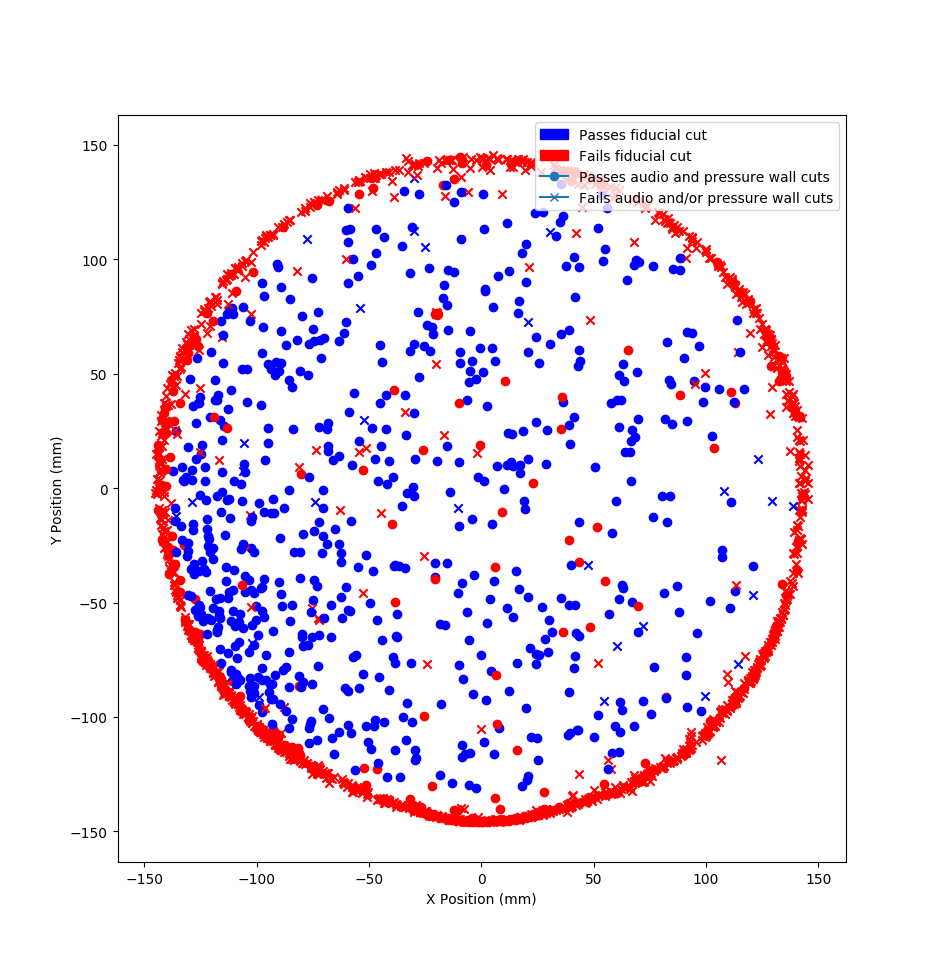
\includegraphics[width=\textwidth]{wall_event_positions}
    \caption{\label{} A visualization of the fiducial cuts and how they match up with the pressure and acoustic cuts.}
\end{figure}

\section{Supervised Learning}

Supervised learning was the first step in the optimization procedure. It makes use of fully labeled calibration sets, which are used for training. Performance of these supervised neural networks is judged based on its accuracy at replication of the provided labels on a validation set (which is set aside and not trained on).

\subsection{Convolutional Neural Network for Raw Waveform Analysis}

A convolutional neural network was used for analyzing the raw waveform $\omega$ directly, without any preprocessing whatsoever. This avoids any destruction of information, and should be possible, in theory, for a neural network to handle. For this task, a very deep 1-dimensional fully convolutional neural network was applied. The architecture was inspired by the M34-res network \cite{verydeepconvnets} for analysis of raw waveforms. L2 regularization was used to alleviate overfitting, and batch normalization was applied to the input. (Its hyperparameters were modified significantly through manual empirical testing as well as grid searches.)

Two different configurations were tested: one that operates strictly on $\omega$ with no position corrections of any kind (furthermore $DeepConv(\omega)$) and one with an additional position input on a lower layer such that it should be able to learn to incorporate position corrections into its outputs ($DeepConvWithPos(\omega, \chi)$). The second configuration was introduced because the position corrections applied to $\beta_{8}$ in previous PICO-60 research were applied only to broad frequency bands and are thus not practical to apply to a full resolution waveform.

During early tests with variations on $DeepConv(\omega)$, it was revealed to have an incredible capability to separate run types based on unwanted biases. It was able to separate the AmBe calibration run from combined background runs with 96\% accuracy, and to separate all calibration runs from background runs with 91\% accuracy. However, during these tests, the white noise at the beginning and hydraulic recompression sounds at the end were not cropped off, and the network was shown to be overfitting on this information.

Once the audio was cropped properly, $DeepConv(\omega)$ achieved a maximum of 77\% accuracy on validation data. Using the same network architecture (except for the input layer), $DeepConvWithPos(\omega, \chi)$ managed 85\%. The maximum obtained on a grid search with position correction was 91\%. While this is not a drastic improvement, it is a fairly strong indication that the network is able to extract meaningful information from the position, which may be used in an internal position correction of the volume. That said, neither of these accuracy statistics are particularly good (graphs of 85\% accuracy often appear effectively random), which does not bode well for this input format as a whole.

\begin{figure}[h]
    \centering
    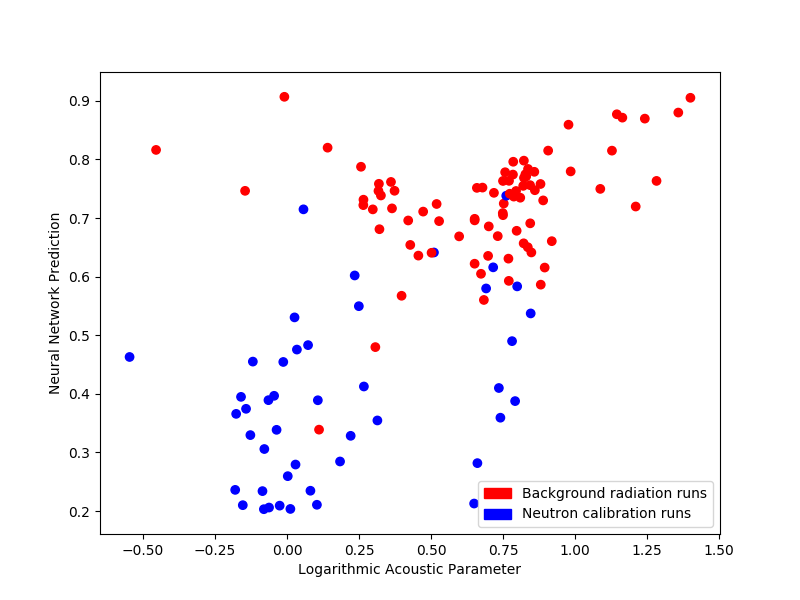
\includegraphics[width=\textwidth]{waveform_best_validation}
    \caption{\label{} Accuracy of $DeepConvWithPos(\omega, \chi)$ compared to Acoustic Parameter at discriminating between run types without $WallCut(D)$.}
\end{figure}

\subsection{Multi-Layer Perceptron for Fourier Transform Analysis}

A multi-layer perceptron (a neural network composed of dense layers) was applied to analysis of audio data in the frequency domain. Preprocessing by applying a Fourier transform makes it an easier task for the neural network to accomplish in some ways. If the frequency distribution and overall volume are indeed the most important factors for discrimination, the network can gather them straight from the Fourier transform $\beta_{N}$ rather than having to analyze $\omega$ to extract this information.

Once again, configurations with and without position input were tested: $FourierMLP(\beta_{N})$ and \\ $FourierMLPWithPos(\beta_{N}, \chi)$. Several different resolutions $N$ of $\beta_{N}$ were used. While there were variety of network architectures tested, most had a small number of layers (on the order of 3), applied dropout and L2 regularization, and used batch normalization once again.

It became evident very quickly that a high resolution was not required to get a high accuracy relative to the ground truth data. A perceptron trained on $\beta_{8}$ managed an excellent 98\% validation accuracy by this metric. Increasing the number of bands seemed initially not to provide any improvement; the best accuracy reached with $\beta_{20}$ was 93\%, and with $\beta_{40}$ it was 94\%.

Unlike for the convolutional neural network trained on $\omega$, wall cuts did not improve performance at all. While $FourierMLP(\beta_{N})$ peaked at 98\% validation accuracy, $FourierMLPWithPos(\beta_{N})$ reached only 95\%. Nevertheless, they both performed better than any of the network architectures trained on $\omega$.

That experimentation applied $WallCut(D)$ to the training and validation sets. Where the higher resolution demonstrated significant power was when $WallCut(D)$ was not applied, and only $QualCut(MultiCut(D))$ was used. The network trained on $\beta_{40}$ still managed 92\% validation accuracy. However, training on $\beta_{50,001}$, which does not incorporate any banding, improved this figure to a maximum of 97\%.

\subsection{Convolutional Neural Network for Image Window Analysis}

It is an open question whether or not there is any information in the image data $\iota$ that could be used to distinguish between particle classes. Relative to the extremely short period of time in which the bubble forms (on the scale of nanoseconds), the framerate of the camera (340Hz) is extremely slow. While the very early stages of bubble formation (when the sound is produced) are known to differ dependong on whether the bubble was created by a nuclear recoil or an alpha particle, it is unknown whether any visually apparent differences persist when the bubble is visible.

In an effort to resolve this, a 2-dimensional convolutional neural network was applied to the task of discriminating based on $\iota$. The network architecture consists of a moderate number of convolutional layers (on the scale of 9) and 3 dense layers at the end. L2 regularization was used on all layers, and dropout was additionally used on the dense layers. No position input is used (since there are no microphones that would require position correction), so the basic configuration is $ImageConv(\iota)$.

Throughout a variety of different network architectures, the best validation accuracy obtained was 85\%. (The corresponding training accuracy of 100\% indicates that severe overfitting is taking place.) It is likely fitting on some form of noise within $\iota$, since the network's predictions seem almost random when represented graphically. The fact that throughout many trials (including a grid search), no good performance on validation data was observed, provides significant evidence that images provide insufficient information for effective discrimination.

\section{Semi-Supervised Learning}

Semi-supervised learning is the idea of training a machine learning model on a set of labeled data in addition to a set of unlabeled data. This has the advantage of requiring fewer labels to be collected than conventional supervised learning. However, it also has a very powerful advantage when training data is impure and the function to be learned is relatively simple (not simple in that it can be easily calculated by a person, but simple in that it does not require a huge set of training data). It allows a neural network to reinforce its own decisions.

In both of the semi-supervised learning algorithms applied, to arrive at an effective discriminator, the network first trains on a smaller amount of imperfect data. Because the ground truth data is imperfect, training on a relatively small set for a short period of time (potentially using regularization, in addition) ensures that the network will be less likely to overfit and its learned function will be simpler. This is in line with the objective, since, assuming the training inputs are normalized correctly, it should be simpler to discriminate between classes of particles than calibration runs.

The essence of this algorithm, then, is a positive feedback loop in which, by using the network's most confident predictions in the training process, the desired (simpler) function is reinforced, when a conventional supervised learning system would have learned the more complex function that is taught by the ground truths.

\subsection{Gravitational Differentiation}

Gravitational differentiation is a novel technique for gradient computation in the final layer of a neural network. It is intended for training a neural network in a semi-supervised fashion on a relatively small set of imperfectly labeled data, while simultaneously incorporating the network's changing predictions on a set of unlabeled data to encourage decisive classifications.

It makes use of the gravitational differentiation function $GravDiff(p, \psi, g)$, which is parameterized by the network's existing prediction $p$ on the training example in question, the degree $\psi$ of the piecewise exponential function used to distort the response of the gradient, and the gravitational multiplier $g$. The function is defined as follows:

$GravDiff(p, \psi, g) = g \cdot sgn(p) \cdot abs(tanh(2(p - 0.5))) ^ \psi$

The essential purpose of $GravDiff(p, \psi, g)$ is to allow confidently classified unlabeled examples to influence the training process, pushing them further towards the classification they are already near (like gravity), while ensuring examples with low-confidence classifications do not have a significant adverse effect.

It can be considered a distortion of the hyperbolic tangent that flattens the central range and exaggerates the asymptote on either side. The network's prediction $p$ is first transformed so its range is 1 to -1 rather than 0 to 1 ($2(p - 0.5)$). Next, the sigmoidal hyperbolic tangent is applied, producing a value of 0 in the center and asymptotic slopes to -1 and 1 at the edges.

However, what is really desired is a shallow slope in the center (so low-confidence network outputs in the range of, for instance, 0.2 to 0.8 will produce very shallow output gradients). Applying a relatively large exponent (on the order of 9) accomplishes this, because values less than 1 will rapidly approach 0. However, this only works with odd integer exponents (because they produce negative outputs for negative inputs), limiting the ability to fine-tune this function by changing $\psi$. To resolve this, a piecewise exponential function is used, where the absolute value is taken prior to applying the power and the sign is multiplied in afterwards. This permits use of the full range of curves produced by even and non-integer values of $\psi$.

This function is applied in a training algorithm that is parameterized by the set of imperfectly labeled data $\varsigma$, the set of unlabeled training data $\upsilon$, a binary classification neural network $NN(x)$ (where $x$ is the input data format), and the gravitational multiplier increment $\delta_g$. The distortion power $\psi$ is assumed to be constant throughout a training run, and the gravitational multiplier $g$ is initialized at 0, gradually increasing during training. It iterates as follows:

\begin{enumerate}
    \item Train $NN(x)$ for a single epoch on the combined set $\varsigma \cup \upsilon$, using the predefined ground truths for $\varsigma$ (with a mean squared error loss function) and the most recently calculated gravitational gradients for $\upsilon$.
    \item Calculate predictions $p$ with $NN(x)$ on the entirety of $\upsilon$. Calculate $GravDiff(p, \psi, g)$ and record the resulting gradients for the next iteration.
    \item Increment $g$ by $\delta_{g}$. At the beginning, when $g = 0$, training will be entirely based on the labeled set $\varsigma$, and progressively, over the course of a run, the gravitational effect increases with $g$.
\end{enumerate}

RESULTS PENDING

\subsection{Iterative Cluster Nucleation}

Iterative cluster nucleation is a semi-supervised learning algorithm that takes advantage of some amount of imperfectly labeled data, using it to classify the rest of an unlabeled training set while optimizing to produce an effective discriminator. The algorithm is initialized as follows:

\begin{enumerate}
    \item Take a subset of the training data, referred to as the seed set $\varsigma$. Use this as the beginning of the training set.
    \item Remove classifications from any other available training examples. These create the unlabeled set $\upsilon$.
    \item Compile and randomly initialize the weights of a binary classification neural network $NN(x)$.
\end{enumerate}

Parameterized by the initial seed threshold $j$ (on the order of 0.01) and the seed threshold multiplier $k$ (on the order of 1.05), the algorithm follows these iterative steps:

\begin{enumerate}
    \item Train $NN(x)$ for 30 epochs on $\varsigma$, using the imperfect ground truth values available.
    \item Using the partially trained weights of $NN(x)$, run inference on the entirety of $\upsilon$, producing a set of predictions $p$.
    \item Find predictions within $p$ that are within a distance of $j$ of either 0 or 1; as this is a binary classifier, such a prediction represents high confidence. Remove any such examples from $\upsilon$ and add them to $\varsigma$. The principle is that, when $NN(x)$ is trained on a relatively small set for short period of time, the few predictions within $p$ that are very confident are highly likely to be correct.
    \item If no examples have been removed from $\upsilon$ and added to $\varsigma$, multiply $j$ by $k$ in place. This is done to increase the acceptance rate later in the training process, when most easily classifiable examples have been added to $\varsigma$. Otherwise, gridlock would occur, where certain examples could not be confidently classified given the training set.
\end{enumerate}

RESULTS PENDING

\section{Technologies}

\subsection{Software}

All programming for this study was done in Python 3. Keras \cite{keras} was used for all machine learning tasks. NumPy and SciPy were used for linear algebra and signal processing. ROOT, scikit-image and scikit-learn were used for data loading and storage. Matplotlib was used for data visualization.

\subsection{Hardware}

Training was done on the Graham supercomputer at the University of Waterloo, accessed through Compute Canada and SHARCNET. I would like to thank Ken Clark and SNOLAB very much for generously providing access to this hardware.

\printbibliography

\end{document}